\documentclass{beamer}
%\documentclass[trans]{beamer}
%\documentclass[handout]{beamer}


\mode<handout>
{
  \usepackage{pgfpages}
  \pgfpagesuselayout{2 on 1}[a4paper,border shrink=5mm]
}

\usetheme{Berlin}
% There are many different themes available for Beamer. A comprehensive
% list with examples is given here:
% http://deic.uab.es/~iblanes/beamer_gallery/index_by_theme.html
% You can uncomment the themes below if you would like to use a different
% one:
%\usetheme{AnnArbor}
%\usetheme{Antibes}
%\usetheme{Bergen}
%\usetheme{Berkeley}
%\usetheme{Berlin}
%\usetheme{Boadilla}
%\usetheme{boxes}
%\usetheme{CambridgeUS}
%\usetheme{Copenhagen}
%\usetheme{Darmstadt}
%\usetheme{default}
%\usetheme{Frankfurt}
%\usetheme{Goettingen}
%\usetheme{Hannover}
%\usetheme{Ilmenau}
%\usetheme{JuanLesPins}
%\usetheme{Luebeck}
%\usetheme{Madrid}
%\usetheme{Malmoe}
%\usetheme{Montpellier}
%\usetheme{PaloAlto}
%\usetheme{Pittsburgh}
%\usetheme{Rochester}
%\usetheme{Singapore}
%\usetheme{Szeged}
%\usetheme{Warsaw}


\usepackage[utf8]{inputenc}
\usepackage[english]{babel}
\usepackage[T1]{fontenc}

\usepackage{amsmath}
\usepackage{amssymb}
\usepackage{amsthm}
\usepackage{enumitem}
\usepackage{minted}
\usepackage{parcolumns}
\usepackage[normalem]{ulem}
\usepackage{tikz}
\usetikzlibrary{shapes,snakes}
\usetikzlibrary{scopes,backgrounds}



\title{Functional Game Programming}

% A subtitle is optional and this may be deleted
%\subtitle{}

\author{David Kr\"{a}utmann, Philip Kindermann}
% - Give the names in the same order as the appear in the paper.
% - Use the \inst{?} command only if the authors have different
%   affiliation.

\institute{RWTH Aachen}
% - Either use conference name or its abbreviation.
% - Not really informative to the audience, more for people (including
%   yourself) who are reading the slides online

% This is only inserted into the PDF information catalog. Can be left
% out. 

% If you have a file called "university-logo-filename.xxx", where xxx
% is a graphic format that can be processed by latex or pdflatex,
% resp., then you can add a logo as follows:

% \pgfdeclareimage[height=0.5cm]{university-logo}{university-logo-filename}
% \logo{\pgfuseimage{university-logo}}
% Let's get started

%tikz
\tikzset{button/.style={draw=red, circle, minimum height=4em}}
\tikzset{block/.style={draw=black, rectangle, minimum width=6em}}
\tikzset{outblock/.style={draw=blue, rectangle split, rectangle split parts=2, minimum width=4em}}
\tikzset{onslide/.code args={<#1>#2}{%
  \only<#1>{\pgfkeysalso{#2}} % \pgfkeysalso doesn't change the path
}}
\tikzset{highlight/.style={draw=blue, text=blue}}

\begin{document}

\begin{frame}
  \titlepage
\end{frame}

\begin{frame}{Why FP?}
    \only<1-3>{
    \begin{itemize}
        \item<alert@+> Declarative approach to programming
        \item<alert@+> What \textit{you want}, not what \textit{to do}
        \item<alert@+> Abstractions \(\Rightarrow\) Increased expressiveness and code reusability
    \end{itemize}}
    
    \begin{minipage}{.49 \textwidth}
     \tiny \inputminted{haskell}{Example.hs}
    \end{minipage}
    \hfill
    \begin{minipage}{.49 \textwidth}
        \tiny \inputminted{python}{example.py}
    \end{minipage}
    
    \only<4->{\begin{tikzpicture}
        \node[button, onslide={<6> highlight}] at (-2,1) (left) {Left};
        \node[button, onslide={<5> highlight}] at (-2,-1) (right) {Right};
        
        \node[block] at (0.5,0) (speed) {speed};
        \node[block, right of=speed, node distance=8em] (integral) {integral 0};
        
        \node[outblock, right of=integral, node distance=8em] (pos) {pos \nodepart{second} {\only<1-4>{0} \only<5>{1} \only<6>{-1.5}}};
        
        \draw [->, onslide={<6> draw=blue}] (left) edge [out=0, in=90] (speed) node [above=10pt, pos=0.25] {\only<6>{2.5s}};
        \draw [->, onslide={<5> draw=blue}] (right) edge [out=0, in=-90] (speed) node [below=10pt, pos=0.25] {\only<5>{1s}};
        
        \draw [->] (speed) -- (integral);
        \draw [->] (integral) edge [out=0, in=90, loop, looseness=4] (integral);
        \draw [->] (integral) -- (pos);
    \end{tikzpicture}}
\end{frame}


\begin{frame}{Functional Reactive Programming}
    \begin{itemize}
        \item Game code always has an iterative component
        \small{\inputminted{haskell}{Loop.hs}}
        \item Task: Handle updates of time-variant data in a composable way
        \item \(\Rightarrow\) Functional Reactive Programming
    \end{itemize}
\end{frame}
\end{document}


